 \documentclass[a4paper,12pt]{article}
 %%%%%%%%%%%%%%%%%%%%%%%%%%%%%%%%%%%%%%%%%%%%%%%%%%%%%%%%%%%%%%%%%%%%%%%%%%%%%%%%%%%%%%%%%%%%%%%%%%%%%%%%%%%%%%%%%%%%%%%%%%%%%%%%%%%%%%%%%%%%%%%%%%%%%%%%%%%%%%%%%%%%%%%%%%%%%%%%%%%%%%%%%%%%%%%%%%%%%%%%%%%%%%%%%%%%%%%%%%%%%%%%%%%%%%%%%%%%%%%%%%%%%%%%%%%%
 \usepackage{eurosym}
 \usepackage{vmargin}
 \usepackage{amsmath}
 \usepackage{multicol}
 \usepackage{graphics}
 \usepackage{enumerate}
 \usepackage{epsfig}
 \usepackage{framed}
 \usepackage{subfigure}
 \usepackage{fancyhdr}
 
 \setcounter{MaxMatrixCols}{10}
 %TCIDATA{OutputFilter=LATEX.DLL}
 %TCIDATA{Version=5.00.0.2570}
 %TCIDATA{<META NAME="SaveForMode" CONTENT="1">}
 %TCIDATA{LastRevised=Wednesday, February 23, 2011 13:24:34}
 %TCIDATA{<META NAME="GraphicsSave" CONTENT="32">}
 %TCIDATA{Language=American English}
 
 %\pagestyle{fancy}
 \setmarginsrb{20mm}{0mm}{20mm}{25mm}{12mm}{11mm}{0mm}{11mm}
 %\lhead{MA4413 2013} \rhead{Mr. Kevin O'Brien}

 
 \begin{document}
 	\tableofcontents

%===================================================%
\section{Introduction}
In this section we aim to replicate the methods proposed by Galecki et al and transfer to them to the
the models fitted by Roy's methodology fitted to the Blood data, as used in Bland and Altman's papers.

%====================================================%
\subsection{nlmeU R package}

This monograph will use functions from the nlmeU package (Galecki and Burzykowski). This package consists of training datasets and utility functions enhancing functionality of nlme package.

\begin{description}
\item[logLik1.lme] Calculates contribution of one subject to the log-likelihood for lme
object

\item[Pwr] Calculates power based on a model fit

\item[sigma] Extract scale parameter sigma from a model fit

\item[simulateY] Simulates values of the dependent variable based on a model fit

\end{description}

%--------------------------------------%
\subsection{ARMD}
Galecki and Burzykowski use in their examples the ARMD data set, sata from Age-Related Macular Degeneration (ARMD) clinical trial. The ARMD data arise from a randomized multi-center clinical trial comparing an experimental treatment (interferon-alpha) versus placebo for patients diagnosed with ARMD.


%====================================================================================%
\newpage
\section{Back Ground Materials}
Galecki and Burzykowski revise several core topics before proceeding to introduce their proposed methodology.

\subsection{Cook's Distance}
%Page 80
% \[ D_i = \frac{ [ \mbox{var}(\hat{\beta})]^{-1} }{\mbox{rank}(\textbf{X})} \]


%====================================================================================%

%Page 497 - Section 20.3
\section{Influence Diagnostics for lme objects.}

\begin{itemize}
\item Cook's Distance
\item Likelihood Distance
\end{itemize}

%------------%
\subsection{Preparatory Steps}

\begin{framed}
\begin{verbatim}
###################################################
### code chunk: Chap20.3influence_init
###################################################

options(width = 65, digits = 5, show.signif.stars = FALSE)
date()
packageVersion("nlmeU")
packageVersion("nlme")
packageVersion("lattice")

sessionInfo()
require(nlme)    
require(lattice) 


data(armd, package="nlmeU")

## Model M16.5 
lm3.form <-                 # (12.9, 16.17)
formula(visual ~ visual0 + time + treat.f) 
fm16.5  <-                  # R16.13
lme(lm3.form,              
random = list(subject = pdDiag(~time)),       
weights =varPower(form=~time),
data = armd)       
\end{verbatim}
\end{framed}

\begin{verbatim}
> summary(fm16.5)
Linear mixed-effects model fit by REML
Data: armd 
AIC  BIC  logLik
6444.9 6483 -3214.5

Random effects:
Formula: ~time | subject
Structure: Diagonal
(Intercept)    time Residual
StdDev:      7.2357 0.28102   5.0391

Variance function:
Structure: Power of variance covariate
Formula: ~time 
Parameter estimates:
power 
0.11052 
Fixed effects: list(lm3.form) 
Value Std.Error  DF  t-value p-value
(Intercept)    5.4416   2.26187 632   2.4058  0.0164
visual0        0.8998   0.03822 231  23.5464  0.0000
time          -0.2416   0.02392 632 -10.0997  0.0000
treat.fActive -2.6553   1.12868 231  -2.3525  0.0195
Correlation: 
(Intr) visul0 time  
visual0       -0.934              
time          -0.071  0.002       
treat.fActive -0.270  0.026 -0.002

Standardized Within-Group Residuals:
Min        Q1       Med        Q3       Max 
-4.148427 -0.329544  0.051823  0.444189  2.930748 

Number of Observations: 867
Number of Groups: 234 
\end{verbatim}
\newpage

\begin{itemize}
\item The \texttt{formula()} can recall the definition of the model defining the mean structure.

\item Auxillary Function \texttt{logLik1()} which is designed to calculate a contribution of a given subject to the overall likelihood for a given model.

\item 
The number of degrees of freedom reported by \texttt{loglik} is equal to 8. This corresponds
to the total number of parameters in the model.
\end{itemize}
%--------------------------------------------%
% Page 498 Top

Part A
\begin{framed}
\begin{verbatim}
	### nlmeU code chunk: R20.6a

	fm16.5ml <- update(fm16.5, method = "ML") # ML estimation
	formula(fm16.5ml)                         # Recall model formula.
	fm16.5ml$call$data                        # Recall data name.
	logLik(fm16.5ml)                          # Log-likelihood value
\end{verbatim}
\end{framed}

\begin{verbatim}
> fm16.5ml <- update(fm16.5, method = "ML") # ML estimation
> formula(fm16.5ml)                         # Recall model formula.
visual ~ visual0 + time + treat.f
> fm16.5ml$call$data                        # Recall data name.
armd
> logLik(fm16.5ml)                          # Log-likelihood value
'log Lik.' -3210.7 (df=8)
\end{verbatim}

%------%

Part B


\begin{framed}
	\begin{verbatim}

	### code chunk: R20.6b

	beta0  <- fixef(fm16.5ml)                 # beta
	names(beta0)                              # Long names
	names(beta0) <- abbreviate(names(beta0), minlength = 7) # Short names 
	beta0                                     # beta printed.
	vcovb  <- vcov(fm16.5ml)                  # vcovb 
	colnames(vcovb) <- names(beta0)           # Short names
	vcovb                                     # vcovb printed. 
	
	
	\end{verbatim}
\end{framed}

\begin{verbatim}
> beta0  <- fixef(fm16.5ml)                 # beta
> names(beta0)                              # Long names
[1] "(Intercept)"   "visual0"       "time"          "treat.fActive"
> names(beta0) <- abbreviate(names(beta0), minlength = 7) # Short names 
> beta0                                     # beta printed.
(Intrc)  visual0     time  trt.fAc 
5.44721  0.89973 -0.24155 -2.65638 
> vcovb  <- vcov(fm16.5ml)                  # vcovb 
> colnames(vcovb) <- names(beta0)           # Short names
> vcovb                                     # vcovb printed. 
(Intrc)     visual0        time     trt.fAc
(Intercept)    5.0475640 -7.9651e-02 -3.8602e-03 -6.8078e-01
visual0       -0.0796512  1.4407e-03  1.5213e-06  1.1239e-03
time          -0.0038602  1.5213e-06  5.6988e-04 -6.1566e-05
treat.fActive -0.6807838  1.1239e-03 -6.1566e-05  1.2568e+00
\end{verbatim}
\newpage
%--------------------------------------------%
% Page 498 Bottom

We extract the \textbf{$\beta$} estimates and their estimated variance covariance matrix.

Towards this end, we use the functions \texttt{fixef()} and \texttt{vcov()} respectively, we can save these estimates and the matrix as objects \texttt{beta0} and 
\texttt{vcovb} respectively.

With the help of the \texttt{abbreviate} function the names of the beta estimates are shortened to simplify the display of content.

%--------------------------------------------%
% Page 499 Top
An auxillary function \texttt{logLik1()}

We used the \texttt{logLik()} function to obtain the value of the log-likelihood for the fitted model.
It should be noted that the function returns the log-likelihood evaluated at the set of the


The auxillary functon \texttt{logLik1()} has been included in the package nlmeU.

estimated fixed effects and variance-covariance parameters and for the data set, to which the model
is fitted. In the context of influence diagnostics, we need a more general function that allows




\begin{description}
\item[ \texttt{modfit} ] an object of class \textit{lme} representing the lme model fited to a given dataset using ML estimation.
\item[ \texttt{dt1}] a dataframe with data for one subject, for whom the likelihood function to be evaluated
\item[ \texttt{dtInit }] an optional auxillary data frame
\end{description}

%--------------------------------------------%
% Page 499 Bottom

The dataframe provided in the argument \texttt{dt1} is typically created by choosing a subset with one subject from the data used to obtain the model fit object specified in the \texttt{modfit} argument.
However, in general, any pluasible fata for one subject , not necessarily from the dataset used to fit the model, can be used.


The auxillary data provided in the argument dtInit is temporarily appended to the dt1 data. during the \texttt{logLik()} function execution.



The \texttt{logLik1()} function returns the numeric contributions of the single subject, with the data specified in the dt1 argument, to the log likelihood
for the model specified in the modfit argument.



% ----------% 
% New Section 
Contributions of Individual Subjects to the log-likelihood for fitted model

%--------------------------------------------%
% Page 500 top

\begin{framed}
	\begin{verbatim}
	###################################################
	### code chunk: R20.7a
	###################################################
	require(nlmeU)  
	df1 <- subset(armd, subject %in% "1")          # Data for subject "1" 
	logLik1(fm16.5ml, df1)                         # logLik_i for subject "1" 
	
	lLik.i <- by(armd, armd$subject,
	FUN = function(dfi) logLik1(fm16.5ml, dfi))
	lLik.i <- as.vector(lLik.i)   # Coerse array to vector  
	lLik.i[1:5]                   # logLik_i for the first five subjects
	sum(lLik.i)                   # Sum logLik_i; compare to Panel 20.6a
	
lLik.i <- as.vector(lLik.i)

lLik.i[1:5]
sum(lLik.i)

\end{verbatim}
\end{framed}
\begin{verbatim}
> df1 <- subset(armd, subject %in% "1")          # Data for subject "1" 
> logLik1(fm16.5ml, df1)                         # logLik_i for subject "1" 
[1] -6.6576
> 
> lLik.i <- by(armd, armd$subject,
+ FUN = function(dfi) logLik1(fm16.5ml, dfi))
> lLik.i <- as.vector(lLik.i)   # Coerse array to vector  
> lLik.i[1:5]                   # logLik_i for the first five subjects
[1]  -6.6576 -13.4708 -11.1361 -13.3109 -12.9930
> sum(lLik.i)                   # Sum logLik_i; compare to Panel 20.6a
[1] -3210.7
> 
> lLik.i <- as.vector(lLik.i)
> 
> lLik.i[1:5]
[1]  -6.6576 -13.4708 -11.1361 -13.3109 -12.9930
> sum(lLik.i)
[1] -3210.7

\end{verbatim}
%-------------------%

Plot of individual contributions to the log-likelihood (traditional graphics)
\begin{framed}
\begin{verbatim}
	
	###################################################
	### code chunk: R20.7b
	###################################################
	nx <- by(armd, armd$subject, nrow)             # ni
	lLik.n <- lLik.i/as.vector(nx)                 # logLiki
	outL <- lLik.n < -6                            # TRUE for values < -6
	lLik.n[outL]                                   # logLiki/ni <  -6
	subject.c <- levels(armd$subject)
	subject.x <- as.numeric(subject.c)
	
	plot(lLik.n ~ subject.x, type = "h")           # Fig. 20.1
	points(subject.x[outL], lLik.n[outL], type = "p", pch = 16)
	text(subject.x[outL], lLik.n[outL], subject.c[outL])
	
\end{verbatim}
\end{framed}
\begin{figure}
\centering
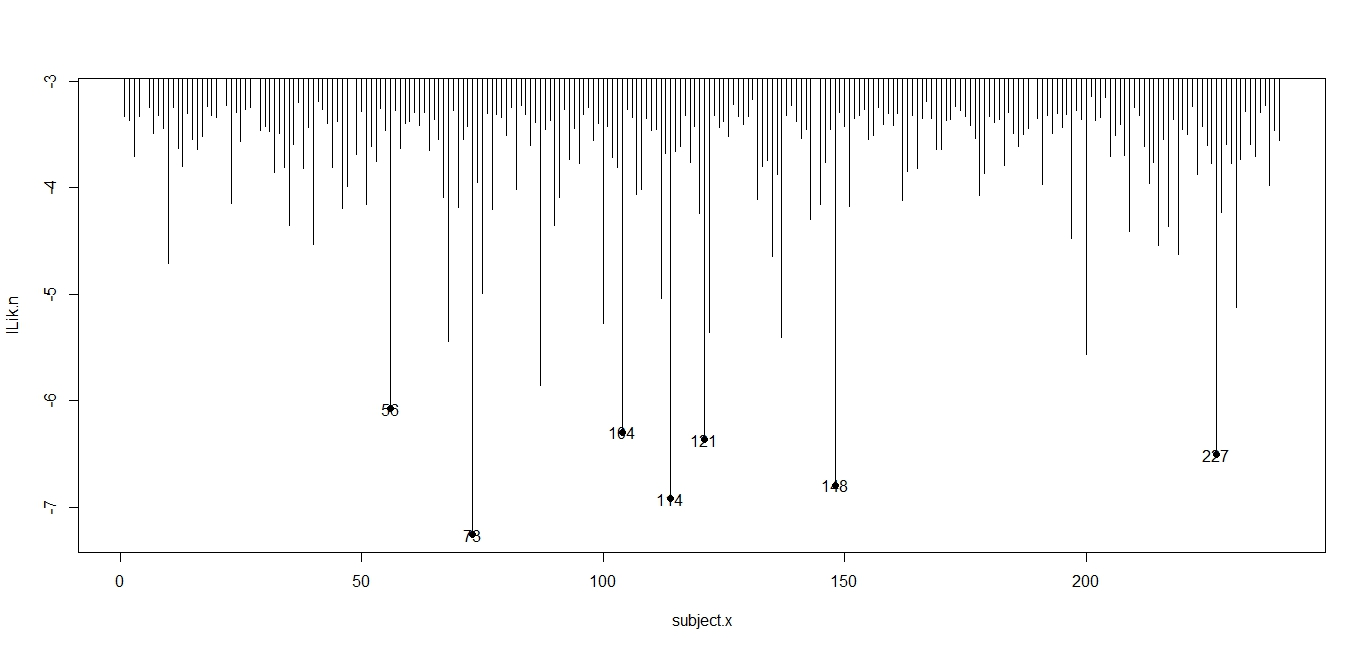
\includegraphics[width=0.7\linewidth]{images/Chap20-image2}
\caption{}
\label{fig:Chap20-image2}
\end{figure}

%--------------------------------------------%
% Page 500 Bottom

next we use the function \texttt{logLik1()} to compute the loglikelihood
contributions for all subjects.

\newpage



	

\newpage
%--------------------------------------------%
% Page 501 top

We present the syntax to plot the per-observation individual log-likelihood contributions.
First, with the help of the \texttt{by()} function, we create the array \texttt{nx} , which contains the number
of observations

%--------------------------------------------%
% Page 501 Bottom

\section{Influence Diagnostics}

We use the results of the preparatory steps to perform influence-diagnostic calculations for the model.
More specifically we evaluate the influence of every subject included in the data set.


We create a list containing the results of fitted model the ``leave-one-subject-out" (LOO)
datasets and explore its contents.

We define the function \texttt{lmeU()}, which fits the model to the data from the armd

when the function \texttt{lmeU()} is executed, and LOO data frame, named dfU, is created with thesubject, indicated by the cx argument.

Subsequently model is fitted by dfI by applying the 


next, with the help of the function \texttt{lapply()}, we apply the \texttt{lmeU()} to the consecutive elements of the character vector subject.c.

As a result, we obtain the list lmeUall, with lme-class model fit objects as elements. The model-fit objects contains the result of fitting model
M16.5.
%--------------------------------------------%
% Page 502 All

Finally, we name the components of the \texttt{lmeUall()} list using the subjects idenifier stored in the vector \textit{subject.c}.

This technique is computationally expensive, as it required the model to be fitted $m$ number of times, omitting one of the $m$ cases each time.

Execution time can be improved if we decided to perform a reduced number of likelihood iterations, instead of performing iterations until there is convergence.

The values, based on the first few iterations, are expected to give a fairly good approximation of the LOO estimates.

%-------%

The names of the first six components are printed out using the function \texttt{names()}.

To extract the LOO data frame for, e.g., the subject ``6", we refer to the ``6" compoment of the
\texttt{lmeUall} list.

The extracted data frame is stored in the object \texttt{dataU6}. By using the function dim() we can check the dimensions of the data frame.



%--------------------------------------------%
% Page 503 Top
Model is fitted to a sequence of "leave-one-subject-out" out data sets.


\begin{framed}
	\begin{verbatim}	
	
	
	###################################################
	### code chunk: R20.8a
	###################################################
	lmeU <- function(cx) { 
	dfU <- subset(armd, subject != cx)          # LOO data 
	update(fm16.5ml, data = dfU)                # LOO fit 
	}
	
	lmeUall        <- lapply(subject.c, lmeU)       # List with LOO fits
	names(lmeUall) <- subject.c                     # Names assigned          
	
	\end{verbatim}
\end{framed}

\begin{framed}
\begin{verbatim}

 # back - what is cx?
 # cx is Case identity
lmeU <- function(cx){
	dfU <- subset(myData, subject !=cx)
	update(mymodel,data=dfU)
}

 # what is lmeU?

lmeUall <- lapply(subject.c, lmeU)
\end{verbatim}
\end{framed}
%------------------------%
Exploring the contents of the lmeUall object.
\begin{framed}
\begin{verbatim}
names(lmeUall)
dataU6 <- lmeUall[["6"]]$data
dim(dataU6)
unique(dataU6$subject)[1:6]
\end{verbatim}
\end{framed}


%-------------------------------------------%
% Page 503 and 504 Bottom
% PArt 20.3.2.2. Likelihood Distacnce for fitted Model
Galecki presents the code used to calculate and plot individial likelihood displacements.

For an LMM, it is required the computation of the full log-likelihood for \textbf{$\hat{\theta}$}, the ML estimate for 
\textbf{$\theta$} obtained by fitting the model to all data, and for \textbf{$\hat{\theta}_(-i)$}, the ML estimate obtained
by fitting the model to the data with the $i-$th subject excluded.

Note that both values of the log-likelihood, used in the definition of the likelihood displacement, should be 
calculated taking into account all observations.

%---------%


Galeck creates an auxillary function \texttt{lLik()} which , for a given subject indicated by the main argument, extracts the lme model fit object for the
corresponding LOO data.


The corresponding log-likelihood function is extracted from the lmeU with the help of the \texttt{logLik()}


The returned value \texttt{lLikU + lLik.s} is the log-likelihood evaluated for all observations, using the displaced estimates of the model parameters.

%------------------------------------------%
% Page 504 Top

Calculation of the likelihood displacement

\begin{framed}
\begin{verbatim}

lLik <- function(cx)
   {
   lmeU <- lmeUall[[cx]]
   lLikU <- logLik(lmeU, REML = FALSE)
   df.s <- subset(armd,subject == cx)
 
   lLik.s <- logLik1(lmeU,df.s)

   return(lLikU + lLik.s)
   }

lLikUall <- apply(subject.c,lLik)

\end{verbatim}
\end{framed}

%--------------------%
% Part 2
% Plot of the likelihood displacement with an indication of outlying values.
%

\begin{framed}
	\begin{verbatim}


###################################################
### code chunk: R20.8b
###################################################
names(lmeUall)[1:6]                             
dataU6 <- lmeUall[["6"]]$data     # LOO data for subject 6
dim(dataU6)                       # Number of rows is 863
unique(dataU6$subject)[1:6]       # Subject no. 6 omitted


###################################################
### code chunk: R20.9a
###################################################
lLik <- function(cx){                  
	lmeU   <- lmeUall[[cx]]           # LOO fit extracted 
	lLikU  <- logLik(lmeU, REML = FALSE)  # LOO log-likelihood
	df.s   <-                         # Data for subject cx...
	subset(armd, subject == cx)                 
	lLik.s <- logLik1(lmeU, df.s)       # ...and log-likelihood.
	return(lLikU + lLik.s)            # "Displaced" log-likelihood...
}
lLikUall <- sapply(subject.c, lLik)     # ...for all subjects.         

dif.2Lik <- 2*(logLik(fm16.5ml) - lLikUall) # Vector of LDi
summary(dif.2Lik)

\end{verbatim}
\end{framed}

\begin{framed}
\begin{verbatim}

names(dif.2Lik) <- subject.c #subjects ids assigned
outL <- dif.2Lik > 0.5

dif.2Lik[outL]

## Plot Component

libary(lattice)

subject.f <- factor(subject.c, levels = subject.c)

myPanel <- function(x,y, ...){
  x1 <- as.numeric(x)
  panel.xyplot(x1,y, ... )
  ltext(x1[outL],y[outL], subject.c[outL]) # outlying LDis
  }

dtp <- dotplot(dif.2Lik ~subject.f, panel = myPanel, type= "h")

 # ggplot?
lxlims <- length(dtp$x.limits)

update(dtp,xlim=rep(" ", lxlims),grid= "h")
\end{verbatim}
\end{framed}

%------------------------------------------%
% Page 505 Top

By applying the \texttt{summary()} function to the vector, we obtain summary statistics of the computed likelihood-displacement values.

we create the logical output vector outL which indicates the subjects with the values of the 
likelihood displacement exceeding say 0.5.

From the printout of the selected elements of the vectir dif.2Lik it follows that there are
seven such subjects.


We then use the function \texttt{dotplot()} from the package lattice to plot the 
likelihood distance value for all subjects.

The x-axis of the plot is constructed using numeric representation of the \texttt{numeric.f} factor, containing values ranging from 1 to 234.

\newpage
\begin{framed}
\begin{verbatim}

###################################################
### code chunk: R20.9b
###################################################
names(dif.2Lik) <- subject.c              # Subjects' ids assigned
outL  <-  dif.2Lik > 0.5                  # Outlying LDi's
dif.2Lik[outL]
library(lattice)
subject.f <- factor(subject.c, levels = subject.c)
myPanel <- function(x, y, ...){
x1 <- as.numeric(x)
panel.xyplot(x1, y, ...)
ltext(x1[outL], y[outL], subject.c[outL])  # Label outlying LDi
}

dtp <-                                        # Fig. 20.2
dotplot(dif.2Lik ~ subject.f, panel = myPanel, type = "h")           
lxlims <- length(dtp$x.limits)         
update(dtp, xlim = rep("", lxlims), grid = "h") 






\end{verbatim}	
	
\end{framed}
%------------------------------------------%
% Page 505 Bottom
\section{20.3.2.3. Cook's Distance for the $\beta$ estimates}

Cook's distance for the $\beta$ estimates was defined in (4.26) for the classical LM.
The definition can be extended to the LMMs in a straightforward manner.

%------------------------------------------%
% Page 506 top

Part 2 plot of cook's distance using traditional graphics

%%% Annotation Component

\begin{framed}
	\begin{verbatim}

###################################################
### code chunk: R20.10a
###################################################
betaUall <- sapply(lmeUall, fixef)          # Matrix with beta(-i)
vb.inv <- solve(vcovb)                       
CookDfun <- function(betaU){  
	dbetaU <- betaU - beta0                  # beta(-i) - beta
	CookD.value <- t(dbetaU) %*% vb.inv %*% dbetaU 
}
CookD.num <- apply(betaUall, 2, CookDfun)
(n.fixeff <- length(beta0))                 # Number of fixed effects
rankX <- n.fixeff                           # Rank of matrix X
CookD <- CookD.num/rankX                    # Cook's distance Di
\end{verbatim}
\end{framed}
%============================================ %
\begin{framed}
\begin{verbatim}
### Blood Data Equivalent
betaUall <- sapply(lmeUall,fixef)

vb.inv <- solve(vcovb)

cookDfun <- function(betaU){
   dbetaU <- betaU - beta0
   cookD.value <- t(dbetaU) %*% vb.inv %*% dbetaU
   }
\end{verbatim}
\end{framed}

%----------------%
Plot of Cook's Distance using traditional graphics. 
Outlying values annotated.

\begin{framed}
\begin{verbatim}

###################################################
### code chunk: R20.10b
###################################################
outD <- CookD > 0.03                        # Outlying Di's
subject.c[outD]                             # Subjects' ids 

plot(CookD ~ subject.c, 
ylab = "Cook's D", type = "h")         # Fig. 20.3
text(as.numeric(subject.c[outD]),
CookD[outD], subject.c[outD])          # Annotation 
points(subject.c[outD], CookD[outD])
\end{verbatim}
\end{framed}



\begin{framed}
\begin{verbatim}
### Blood Data Equivalent
outD <- cookD > 0.03


#Create the Stick plot
plot(CookD ~ subject.c, 
  ylab="Cook's Distance", type="h")

text()
points()
\end{verbatim}
\end{framed}

%------------------------------------------%
% Page 506 bottom 
Cook's distance for the $beta$ estimates were defined bu 4.26 for the classical LM model.


Next we compute the inverse of the variance covariance matrix $\hat{\beta}$ using the \texttt{solve()} function.
We store the resulting matrix in the object \texttt{vb.inv}.

Subsequently we define the function \texttt{cookDfun()} which, for a vector given in
the \texttt{betaU} argument, computes the value of the numerator of Cook's Distance, as in (4.26).

The function is then applied sequentially to all columns of the matrix \texttt{betaUall}.


The resultant vector is divided by the number of the fixed effects coefficients, which, under the assumption that the design matrix is of full rank, 
is equivalent to the rank of the design matrix.

%------------------------------------------%
% Page 507 all


The outcome is stored in the vector \texttt{cookD} and contains the values of cooks distanced for all subjects.

We create the logical vector outD which indicates the subjects with cook's distance values that exceed 0.03.

Present the scatterplot matrix of the two-dimensional projections of the differences.
% \[  \frac{\hat{\textbf{beta}_{(-i)} - \hat{\textbf{beta}} }{\hat{se}(\hat{beta})} \]
for all pairs of the fixed-effects coefficients.

%-------%
The plot was generated using the \texttt{splom} function. The main argument of the 
function was obtained by subtracting the beta0 vector from the rows of the transposed
betaUall matrix.

%-------%
The labels used in the panels located on the diagonal of the figure provide the fixed estimates of fixed effects coefficients
of the model and their estimates SEs.
The panels above the diagonal include points for all subjects.
The points for non-outlying values are plotted using small size open circles.
The five outlying values are plotted using different plotting symbols defined in the
legend of the figure at the top of the graph.

%------------------------------------------%
% Page 508 All +  top of Page 509

The effect of removal of this subject on the estimates of the remaining fixed-effects coefficients is relatively small.
In contrast, removing the subject ``227" affects the estimate of all fixed-effects coefficients to a different degree and in different directions.

More specifically, the intercept is driven towards lower values : the positive slope associated with visual acuity at baseline visual0, is further increased, the negative slope associated with \texttt{time} is brough closer to zero, and the treatment effect is attenuated.

% Top of Page 509

Overall we note that the effect of removing any of the subjects on the fixed effects estimates is very small, as it does not exceed 0.05 of the SE of any of the  estimates.

%-------------------------------------------%
%Page 509 Top
\newpage
\section{Simulation of the Dependent Variable}

\begin{verbatim}
### Note: Simulations in Panel R20.11 take a long time

###################################################
### code chunk: Chap20.4init
###################################################
options(width = 65, digits = 5, show.signif.stars = FALSE)
date()

sessionInfo()

require(nlme)    #

data(armd, package="nlmeU")

lm3.form   <-                           # (12.9)
formula(visual ~ visual0 + time + treat.f) 
fm16.5  <-     #update(fm16.4,          # M16.5 <- M16.4           
lme (lm3.form, 
random = list(subject = pdDiag(~time)),
weights = varPower(form = ~time), # 
data = armd)            
fm16.5ml <- update(fm16.5, method = "ML")


###################################################
### code chunk: R20.11
###################################################
library(nlmeU)
simY <- simulateY(fm16.5ml, nsim = 1000, seed = 1238917)  # Simulated y from M16.1
auxDt <- subset(armd,                    # Auxiliary data
select = c(subject, visual, visual0, time, treat.f))
simYsumm <- 
apply(simY, 
MARGIN = 2,                     # Over columns
FUN = function(y){    
auxDt$visual <- y            # Dependent variable updated
auxFit <-                    # Update M16.1 with new y
update(fm16.5ml, data = auxDt)
summ <- summary(auxFit)      # Summary
beta <- fixef(summ)     
list(beta = beta)
})
simYsumm[[1]]                            # beta for the 1st simulation


###################################################
### code chunk: R20.12
###################################################
betaE <- sapply(simYsumm,            # Matrix with betas
FUN = function(x) x$beta)
rowMeans(betaE)                      # Empirical beta (see Panel R20.6b)
cov(t(betaE))                        # Emoirical Var(beta)

## sessionInfo
sessionInfo()
\end{verbatim}
We cosnider simualtions of the dependent variable, based on the marginal distribution 
implied by the fitted model.
Towards this end, we have developed \texttt{simulateY()}, which can be used for objects of class lme.

We note that the function is different from simulate.lme(), available in the nlme in that the latter returns
simulation-based REML and/or ML values and not the value of the dependent variable.

We demonstrate the use of the \texttt{simulateY()} function to create the empirical distribution of the \textbf{$\beta$} estimates.
As an example, we consider the model which was fitted to the armd data.

Note however that the presented syntax is fairly general can be used for other LMEs as well.

We apply the function \texttt{simulateY()} to the object fm16.5ml.


%-------------------------------------------%
%Page 509 Bottom

\begin{framed}
\begin{verbatim}
library(nlmeU)
simY <- simulateY(fm16.5ml, nsim=1000)


simYsumm <- apply( simY, MARGIN = 2, 
 FUN = function(y){

     }
   )


simYsumm[[1]]

# \hat{\beta} for the 1st simulation
\end{verbatim}
\end{framed}
%--------------------------------------------%
% Page 510 Top

There is a second argument \texttt{nsim} that indicated how many simulations 

The auxillary function performs the following steps

\begin{itemize}
\item the dependent variable visual is the \texttt{auxDt} data frame is replaced wiht a new set of simulated values contained in the vector $y$.
\item Model M16.5 is fitted to the modified data frame
\item the vector beta with the estimates of the fixed effects coefficients is extracted from the summary of the model-fit object with the help of the \texttt{fixef()} function.
\item The vector of estimates is returned as a list with one component named \texttt{beta}.
\end{itemize}

They are drawn from the marginal distribution of the dependent variable implied by the fitted model.

%--------------------------------------------%
% Page 510 Bottom


It should be mentioned that the creation of the simYsumm list involves refitting the model many times, and it therefore takes a long time.

Toward this end, with the help of the \texttt{sapply()} function, we extrac the vectors with the values of $\hat{\beta}$ for each simulation for the list
-object \texttt{simYsumm} and bind them column-wise into the \texttt{betaE}.

Then we use the function \texttt{rowMeans()} to compute the mean values of the columns (i.e. accross the rows) of betaE.



%--------------------------------------------%


\end{document}
